\begin{frame}{¿Qu\'e otros escenarios ser\'ia interesante modelar?}
    \begin{block}{}
        Dentro de los {\color<2>{orange}jugadores} existen dos clases especiales de jugadores:
        \begin{itemize}
            \item   Los {\color<2>{orange}jugadores premium}
             son aquellos que se han gastado dinero en el juego, de estos se almacena
            la {\color<2>{attr}cantidad de dinero que han gastado} y su m\'etodo de pago preferido.

            \item  Los {\color<2>{orange}jugadores profesionales} son aquellos que {\color<2>{blue}son miembros} de un
            {\color<2>{orange}equipo profesional} y de ellos se almacena su {\color<2>{attr}ranking}.
        \end{itemize}
        De un equipo profesional se conoce su {\color<2>{attr}identificador}, 
        {\color<2>{attr}nombre} y {\color<2>{attr}pa\'is} de origen.
      
        
     
    \end{block}
\end{frame}

\begin{frame}{Especializaci\'on y generalizaci\'on}
    \begin{block}{Especializaci\'on}
        Subconjunto de otro conjunto de entidades
        \vspace{5mm}

        \centering
        
\begin{tikzpicture}
            \node[align=left] at (0,0) {J. PREMIUM\\J. PROFESIONAL};
            \draw [decorate,thick,decoration = {brace}] (1.6,0.5) --  (1.6,-0.5);
            \draw [->, thick] (1.7,0) -- (5,0) node[midway,above] {\small Especializaci\'on};
            \node at (6,0) {JUGADOR};
        \end{tikzpicture}
    \end{block}

    


    \begin{block}{Generalizaci\'on}
        Superconjunto de otro conjunto de entidades
        \vspace{5mm}

        \centering
        
\begin{tikzpicture}
            \node[align=left] at (6.1,0) {J. PREMIUM\\J. PROFESIONAL};
            \draw [decorate,thick,decoration = {brace, mirror}] (4.5,0.5) --  (4.5,-0.5);
            \draw [->, thick] (1,0) -- (4.4,0) node[midway,above] {\small Generalizaci\'on};
            \node at (0,0) {JUGADOR};
        \end{tikzpicture}
    \end{block}


    

\end{frame}


\begin{frame}{Especializaci\'on y generalizaci\'on}
    \centering
    \resizebox{!}{6cm}{
    \begin{tikzpicture}[node distance=5em]
                \tikzset{link/.append style={
            postaction={decorate},
            decoration={
                markings,
                mark= at position 0.5 with {
                    \draw (0.5em,1ex) -- (-0.5em,1ex) to[bend right=90] (-0.5em,-1ex) -- (0.5em,-1ex);
                }
            }
        }}
        \tikzstyle{every entity} = [minimum width=2cm, minimum height=0.8cm]

        \node[entity] (jugador) {\small JUGADOR}
            [sibling distance=3cm]
            child {node[attribute] [above left of=jugador] {\tiny NIVEL}}
            child {node[attribute] [above right of=jugador]{\tiny TROFEOS}}
            child {node[attribute] [above of=jugador] {\tiny TROFEOS MAX}}
            child {node[attribute] [right of=jugador]{\tiny APODO}}
            child {node[attribute] (ci) [left of=jugador] {\tiny \underline{CI}}};


        \node[entity] (premium) at (-2,-3) {\small J. PREMIUM}
            [sibling distance=2.5cm]
            child {node[attribute] [below left of=premium] {\tiny GASTO T.}}
            child {node[attribute] [below right of=premium] {\tiny M. PAGO}}
            child {node[attribute, dashed] [left of=premium] {\tiny \underline{CI}}};

        \node[entity] (profesional) at (2,-3) {\small J. PROFESIONAL}
            [sibling distance=3.2cm]
            child {node[attribute, dashed] [below left of=profesional] {\tiny \underline{CI}}}
            child {node[attribute] [below right of=profesional] {\tiny RANKING}};

        \draw[link] (premium.north) -- (-2,-1.3);
        \draw[link] (profesional.north) -- (2,-1.3);
        \draw (jugador.south) -- (0,-1.3);
        \draw (-2,-1.3) -- (0,-1.3);
        \draw (2,-1.3) -- (0,-1.3);
        % \draw[link] (premium.north) -- (jugador.south);
        % \draw[link] (profesional.north) -- (jugador.south);

        \node[entity] (equipo) at (9,-3) {\small EQUIPO}
        [sibling distance=3cm]
        child {node[attribute] [above left of=equipo] {\tiny \underline{EQUIPO\_ID}}}
        child {node[attribute] [above of=equipo] {\tiny NOMBRE}}
        child {node[attribute] [above right of=equipo] {\tiny PA\'IS}};
        \node[relationship, aspect=2] (miembro) at (5.8,-3) {\small MIEMBRO} edge(profesional) edge(equipo);
        \node at (3.9,-2.8) {\small $1,\ast$};
        \node at (7.6,-2.8) {\small $1,1$};


    \end{tikzpicture}
    }
\end{frame}


% @TODO kita estos frames de herencia
\begin{frame}{Herencia de atributos e interrelaciones}
    \centering

    \resizebox{14cm}{!}{
    \begin{tikzpicture}
        \node[align=left] at (0,0) {\hspace{22mm}\small  JUGADOR\\ \{(98012300205, Juan, 1, 1800, 2300),...\}};
        \node[align=left] at (8,0) {\hspace{25mm}\small  ENFRENTAR\\ \{(98012300205, 97041223987, 24/02/23-14:55),...\}};
        \node[align=left] at (3,-3) {\small J. PROFESIONAL \{(98012300205, 100),...\}};
        \node[align=left] at (3,-6) {\small MIEMBRO \{(98012300205, 1),...\}};

        \only<2>{
            \draw[->,color=red] (3,-2.8) -- (-2,-0.4) node[midway, above right] {Atributos heredados};
            \draw[->,color=red]  (4.3,-4) --  (5.3,-3.2) node[midway, below right] {Atributos espec\'ificos};
        }
        
        \only<3>{
            \draw[->,color=red] (3.5,-2.8) -- (5.6,-0.4) node[midway, below right] {Interrelaci\'on heredada};
            \draw[->,color=red] (3.5,-3.2) -- (3.5, -5.8) node[midway, right] {Interrelaci\'on espec\'ifica};
        }
    \end{tikzpicture}
    }
\end{frame}

\begin{frame}{Modelando tipos de cartas}
    Las {\color<2>{orange}cartas} se clasifican en tres tipos principales: hechizo, tropa
    y estructura.
    \begin{itemize}
        \item De los {\color<2>{orange}hechizos} se conoce el {\color<2>{attr}radio de efecto},
        su {\color<2>{attr}duraci\'on},
        el {\color<2>{attr}da\~no en \'area} y el {\color<2>{attr}da\~no a las torres enemigas}.
        \item De las {\color<2>{orange}tropas} se conocen sus {\color<2>{attr}puntos de vida}, el {\color<2>{attr}da\~no en \'area} y
        la {\color<2>{attr}cantidad de unidades} que tiene.
        \item De las {\color<2>{orange}estructuras} se conocen sus {\color<2>{attr}puntos de vida}, el {\color<2>{attr}da\~no a distancia}
        y la {\color<2>{attr}velocidad de ataque}.
    \end{itemize}
\end{frame}

\begin{frame}{Especializaci\'on por partici\'on}
    \centering
    \resizebox{!}{6cm}{
    \begin{tikzpicture}[node distance=6em]
        \tikzset{link/.append style={
            postaction={decorate},
            decoration={
                markings,
                mark= at position 0.5 with {
                    \draw (0.5em,1ex) -- (-0.5em,1ex) to[bend right=90] (-0.5em,-1ex) -- (0.5em,-1ex);
                }
            }
        }}
        \tikzstyle{every entity} = [minimum width=2cm, minimum height=0.8cm]
        \node[entity] (carta) at (0,0) {CARTA}
        [sibling distance=3cm]
        child {node[attribute] [above left of=carta] {\tiny CALIDAD}}
        child {node[attribute] [above right of=carta]{\tiny DESC.}}
        child {node[attribute] [above of=carta] {\tiny NOMBRE}}
        child {node[attribute] [right of=carta]{\tiny COSTO}}
        child {node[attribute] [left of=carta] {\tiny \underline{CARTA\_ID}}};
        \node[regular polygon, draw, regular polygon sides=6, minimum width=7mm, xscale=3, label=center:TIPO] (tipo) at (0,-2) {};
        \draw (carta.south) -- (tipo.north);
        \node[entity] (tropa) at (0,-4.5) {TROPA}
        [sibling distance=3cm]
        child {node[attribute, dashed] [above left of=tropa] {\tiny \underline{CARTA\_ID}}}
        child {node[attribute] [below of=tropa] {\tiny P. VIDA}}
        child {node[attribute] [below right of=tropa] {\tiny D. \'AREA}}
        child {node[attribute] [above right of=tropa] {\tiny UNIDADES}};
        \node[entity] (hechizo) at (-4,-4.5) {HECHIZO}
        [sibling distance=3cm]
        child {node[attribute, dashed] [left of=hechizo] {\tiny \underline{CARTA\_ID}}}
        child {node[attribute] [below left of=hechizo] {\tiny RADIO}}
        child {node[attribute] [below of=hechizo] {\tiny DURACI\'ON}}
        child {node[attribute] [below right of=hechizo] {\tiny D. \'AREA}}
        child {node[attribute] [above left of=hechizo] {\tiny D. TORRES}};
        \node[entity] (estructura) at (3.4,-4.5) {ESTRUCTURA}
        [sibling distance=3cm]
        child {node[attribute, dashed] [above right of=estructura] {\tiny \underline{CARTA\_ID}}}
        child {node[attribute] [right of=estructura] {\tiny D. DIST}}
        child {node[attribute] [below of=estructura] {\tiny V. ATAQUE}}
        child {node[attribute] [below right of=estructura] {\tiny P. VIDA}}
        ;
        \draw[link] (tropa.north) -- (tipo.south);
        \draw (-4,-2) -- (-1,-2);
        \draw[link] (hechizo.north) -- (-4,-2); 
        \draw (3.4,-2) -- (1,-2);
        \draw[link] (estructura.north) -- (3.4,-2);
    \end{tikzpicture}
    }
    \vspace{5mm}

    \centering
    \textcolor{red}{\Large Los conjuntos de entidades especializados son disjuntos}
\end{frame}


\begin{frame}{Modelando el juego competitivo}
    Las competencias para equipos profesionales se denominan {\color<2>{orange}ligas profesionales}, 
    de las que se conoce su {\color<2>{attr}identificador}, {\color<2>{attr}nombre} y 
    {\color<2>{attr}patrocinador}.
    Las ligas {\color<2>{blue}organizan} una nueva {\color<2>{orange}temporada} cada a\~no, de las cuales se conoce el 
    {\color<2>{attr}a\~no en
    que se realiz\'o}, el {\color<2>{attr}premio por ganar la liga}, y los {\color<2>{orange}equipos} que 
    {\color<2>{blue}participaron}. 
\end{frame}

\begin{frame}{¿Pueden encontrar el problema?}
    \tikzstyle{every entity} = [minimum width=2.3cm, minimum height=1.2cm]
    \centering
    \resizebox{!}{7.5cm}{
    \begin{tikzpicture}[node distance=6em]
        \node[entity] (liga) at (0,0) {LIGA}
        [sibling distance=3cm]
        child {node[attribute] [above of=liga] {\tiny NOMBRE}}
        child {node[attribute] [above right of=liga] {\tiny PATROCINADOR}}
        child {node[attribute] [above left of=liga] {\tiny \underline{LIGA\_ID}} };
        \node[entity] (temp) at (0,-5) {TEMPORADA}
        child {node[attribute] [below of =temp] {\tiny A\~NO}}
        child {node[attribute] [below right of=temp] {\tiny PREMIO}};
        \node[entity] (equipo) at (9,-5) {EQUIPO};
        \node[relationship,aspect=2] (organizar) at (0,-2.5) {ORGANIZAR} edge(liga) edge(temp);
        \node[relationship,aspect=2] (competir) at (4.5,-5) {COMPETIR} edge(temp) edge(equipo); 

        \node at (0.4,-1) {$1,1$};
        \node at (0.4,-4.1) {$1,\ast$};
        \node at (1.7,-4.8) {$1,\ast$};
        \node at (7.4,-4.8) {$\ast,\ast$};
    \end{tikzpicture}
    }
\end{frame}


\begin{frame}{El problema}
    \centering
    \begin{tikzpicture}[node distance=5em]
        \node[entity] (temp) at (0,0) {TEMPORADA}
            [sibling distance=3cm]
            child {node[attribute] [above left of=temp] {\tiny A\~NO}}
            child {node[attribute] [above right of=temp] {\tiny PREMIO}};
    \end{tikzpicture}
    \vspace{5mm}

    \centering
    \textcolor{red}{\Large ¿Qu\'e atributo seleccionar como llave de TEMPORADA?}

    
\end{frame}

\begin{frame}{Conjuntos de entidades fuertes y d\'ebiles}
    \begin{block}{Conjunto de entidades fuerte}
        Sus instancias se pueden identificar
        un\'ivocamente independientemente del resto de los conjuntos de entidades.
    \end{block}

    \begin{block}{Conjunto de entidades d\'ebil}
        Su existencia depende de la existencia
        de otro conjunto de entidades. El identificador de la entidad
        d\'ebil es un superconjunto
        del identificador de la entidad fuerte de la cual depende.
    \end{block}
\end{frame}



\begin{frame}{Conjuntos de entidades fuertes y d\'ebiles}
    \tikzstyle{every entity} = [minimum width=2.3cm, minimum height=1.2cm]
    \centering
    \resizebox{!}{7.5cm}{
    \begin{tikzpicture}[node distance=6em]
        \node[entity] (liga) at (0,0) {LIGA}
        [sibling distance=3cm]
        child {node[attribute] [above of=liga] {\tiny NOMBRE}}
        child {node[attribute] [above right of=liga] {\tiny PATROCINADOR}}
        child {node[attribute] [above left of=liga] {\tiny \underline{LIGA\_ID}} };
        \node[entity,double distance =1.5 pt] (temp) at (0,-5) {TEMPORADA}
        child {node[attribute,dashed] [below left of=temp] {\tiny \underline{LIGA\_ID}} }
        child {node[attribute] [below of =temp] {\underline{\tiny A\~NO}}}
        child {node[attribute] [below right of=temp] {\tiny PREMIO}};
        \node[entity] (equipo) at (9,-5) {EQUIPO};
        \node[relationship,aspect=2,double distance =1.5 pt] (organizar) at (0,-2.5) {ORGANIZAR} edge(liga) edge(temp);
        \node[relationship,aspect=2] (competir) at (4.5,-5) {COMPETIR} edge(temp) edge(equipo); 

        \node at (0.4,-1) {$1,1$};
        \node at (0.4,-4.1) {$1,\ast$};
        \node at (1.7,-4.8) {$1,\ast$};
        \node at (7.4,-4.8) {$\ast,\ast$};
    \end{tikzpicture}
    }
\end{frame}

% \begin{frame}{En resumen}
%     \begin{itemize}
%         \item Un MERX permite representar de forma visual una base de datos
%         que soluciona los requerimientos informacionales de determinado fen\'omeno
%         \item El MERX es un modelo generalmente subjetivo pero: \begin{itemize}
%             \item Existen MERX objetivamente malos
%             \item Existen MERX objetivamente buenos 
%         \end{itemize}
%         \item Pueden existir m\'ultiples MERX que satisfacen los requerimientos informacionales
%         \item El MERX tienen sus limitaciones y existirán restricciones que no puedan ser representadas con el MERX
%     \end{itemize}
% \end{frame}



% \begin{frame}
%     Esta diapositiva deberia tener alguna foto que comparta un sentimiento
%     de realizaci\'on al terminar una tarea ya que por fin terminamos la modelaci\'on
% \end{frame}

% \begin{frame}
%     Esta diapositiva debe contener capturas de pantalla de la orden
%     del problema redactada en lenguaje natural para que vean de donde partimos
% \end{frame}

% \begin{frame}
%     MERX final completo para que vean a qu\'e llegamos
% \end{frame}


  